\section{Quantitative analysis}\label{sec:quant}

% TODO(BH): draft framing. The design counterfactuals (all already
% computed by the pipeline; figures regenerate via
% pipeline/dynamic_game/run_experiments.py, run_extension.py,
% run_deductible_frontier.py):
%
% 1. Attacker-amplified moral hazard: full mechanism vs no-forfeiture vs
%    no-insurance (h* 1.16 -> 0.18; hacks 2.3 -> 10.8/yr).
% 2. The coverage-security frontier and the decoupling escape (Prop. D):
%    fig_decoupling.
% 3. Endogenous pool alpha: carry extinction vs security (capital
%    efficiency frontier in K).
% 4. eta sweep: who is attacked and the system loss rate as the cost
%    technology varies.
% 5. Frontier validation: re-estimating (kappa, eta) from simulated
%    equilibrium incidents (estimator recovers eta with the predicted
%    downward bias).
% TODO(BH): report each counterfactual in percent / dollar terms
% (per positioning_memo.md §5 -- the Ma-Zeng-Zhang configuration).

\begin{figure}[t]
  \centering
  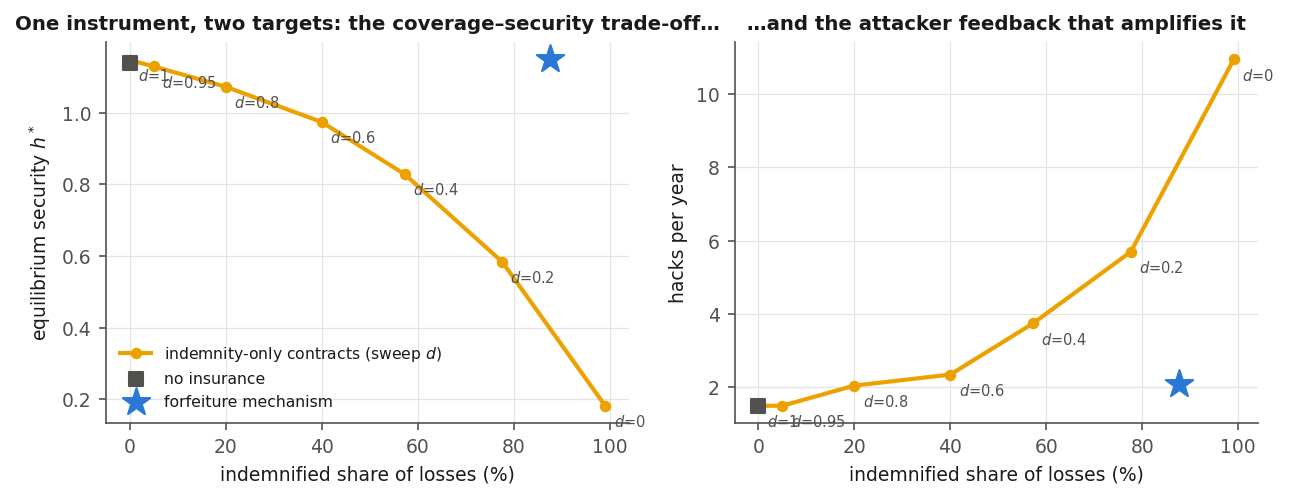
\includegraphics[width=\textwidth]{figures/fig_decoupling.png}
  \caption{The coverage--security frontier of indemnity-only contracts
  (coinsurance $d$ swept from full indemnity to full denial; orange) and
  the forfeiture mechanism (blue star), which attains near-full transfer
  at the no-insurance security level. Left: equilibrium security $h^*$;
  right: realized hack intensity. \emph{[TODO(BH): final caption.]}}
  \label{fig:decoupling}
\end{figure}

\emph{[To be drafted.]}
